\chapter{Experiments}
\label{chap:ch4}

\section{Dataset}
\label{sec:ch4sec1}

The experiments were conducted on a dataset generated using the TPC-H benchmark tool \texttt{dbgen}, which simulates a large-scale business environment for decision support systems. The dataset size used in this study is approximately 1 GB, providing a realistic volume for performance evaluation in database-intensive software product lines (SPLs).

To accommodate the SPL context, the original TPC-H schema was extended with additional tables representing feature-specific modules such as \textit{customer loyalty}, \textit{newsletter subscription}, and \textit{purchase summary}. These extensions enable the evaluation of modular and flat database architectures reflecting different SPL configurations.

The dataset includes the following key tables relevant to the experiments:
\begin{itemize}
    \item \textbf{CUSTOMER} and \textbf{ORDERS}: Core TPC-H tables representing customers and their orders.
    \item \textbf{LINEITEM} and \textbf{PART}: Supporting tables for detailed order and product information.
    \item \textbf{CUSTOMER\_LOYALTY}, \textbf{CUSTOMER\_NEWSLETTER}, and \textbf{CUSTOMER\_PURCHASE\_SUMMARY}: SPL extension tables capturing feature-specific data.
\end{itemize}

Data population scripts and transformations were applied to reflect feature-specific logic, such as loyalty point calculations and newsletter subscription statuses. The resulting dataset supports benchmarking of different SPL testing approaches and database schema evolution strategies as explored in this work.


\section{Experimental Setup}
\label{sec:ch4sec2}

The experiments were carried out on a system equipped with an AMD Ryzen 5  processor, 16 GB of RAM, and SSD storage, running Windows 11. The database server used was MySQL Server version 8.0, hosting an extended TPC-H benchmark dataset of approximately 1 GB. This dataset was enhanced with additional tables representing software product line (SPL) features such as customer loyalty, newsletter subscriptions, and purchase summaries.

The testing framework was developed in Python 3.10, leveraging the \texttt{pytest} testing library to automate query executions corresponding to different SPL feature variants: \textit{loyalty}, \textit{newsletter}, and \textit{full}. Each variant selectively enables or disables tests to simulate feature-specific behaviors and adaptations.

Queries were executed multiple times to mitigate transient system variability, with execution durations recorded using Python's timing utilities. The database schema included appropriate indexing on key columns to reflect realistic optimization conditions and to ensure fairness across benchmarks.

\section{Analysis Metrics}
\label{sec:ch4sec3}

This section presents the key performance and correctness metrics used to evaluate the experiments across the three papers studied. The goal is to provide a consistent and objective basis for comparing the different SPL testing approaches and database adaptations.

\subsection{Execution Time}

The primary metric for performance evaluation is the \textbf{execution time} of SQL queries or test cases. For the first two papers, execution time was measured by manually running the SQL queries against the database and recording the duration taken to complete each query. For the third paper, the Python testing framework logged the time taken for each test case execution using \texttt{pytest}'s built-in timing facilities.

Execution times are reported in seconds and averaged over multiple runs to mitigate variability caused by transient system load or caching effects. This metric reflects the practical efficiency of different query formulations, schema designs, and testing approaches.

\subsection{Explain Plan Analysis}

To complement raw execution times, \textbf{query execution plans} (explain plans) were analyzed to understand the internal operations performed by the database engine. Explain plans provide insights into the indexes used, join methods, and estimated rows processed, which helps interpret the performance differences observed.

\subsection{Correctness and Test Outcomes}

For the automated Python testing suite, correctness was evaluated through the pass/fail status of individual test cases. Tests were designed to assert expected query results and validate schema consistency. The aggregated test results provide a qualitative measure of the reliability of the SPL testing methods.

\subsection{Result Logging and Statistical Analysis}

All performance and correctness data were exported into CSV files for systematic aggregation. Statistical measures such as mean, median, and standard deviation of execution times were computed to summarize the results. These statistics form the basis for comparing performance trends across different experimental configurations.

\subsection{Limitations of Metrics}

While execution time and explain plan analysis offer valuable performance insights, they may be influenced by factors outside the scope of this study, such as hardware variability and concurrent system processes. Correctness assessments depend on the completeness of the test suite and may not capture all edge cases. These limitations are discussed further in Section~\ref{sec:ch4_threats}.




\section{Results}

This section presents the findings from the three experimental setups conducted to evaluate various Software Product Line (SPL) testing approaches inspired by the selected papers. We report query execution times, explain plans, and automated test results, highlighting performance differences and insights.

\subsection{SPL-DB-Sync Benchmark Results}

The first experiment focused on the SPL-DB-Sync \cite{P6} approach, where we benchmarked modular and flat architectural variants across three SPL feature modules: loyalty, newsletter, and purchase summary.

\begin{itemize}
    \item \textbf{Loyalty Program Module:} The modular (JOIN) approach achieved consistent query execution times around 0.015 seconds, while the flat approach was slightly slower, with fetch times around 0.062 seconds. Explain plans showed efficient index usage in the modular variant.
    \item \textbf{Newsletter Module:} Similar patterns were observed, with modular queries running between 0.015 and 0.032 seconds, and flat queries slightly slower (~0.047 seconds). Indexes on the foreign key columns contributed to this performance.
    \item \textbf{Purchase Summary Module:} This module showed the most notable difference, with modular query durations below 0.2 seconds but flat queries consistently exceeding 14 seconds, primarily due to the lack of indexes and the use of temporary tables, as indicated in explain plans.
\end{itemize}

These results demonstrate that modular database transformations can significantly improve query performance in SPL environments, especially for complex aggregations.

\subsection{AMOEBA Query Performance Results}

The second experiment evaluated query pairs from the AMOEBA paper \cite{P3}, focusing on different SQL formulations for equivalent operations.

\begin{itemize}
    \item \textbf{Query Pair 1 (Order Price Threshold):} The JOIN-based query (1B) executed significantly faster (~0.018 seconds) than the nested IN query (1A) which took over 1.5 seconds on average.
    \item \textbf{Query Pair 2 (Order Date Filter):} The JOIN variant again outperformed the EXISTS-based query, running in under 0.02 seconds compared to over 1.3 seconds.
    \item \textbf{Query Pair 3 (Total Spent Calculation):} The scalar subquery (3A) performed very efficiently (~0.015 seconds), whereas the GROUP BY with JOIN (3B) took over a minute due to the large dataset and the aggregation overhead.
    \item \textbf{Query Pair 4 (Expensive Products Filter):} Multi-level JOIN (4B) queries were much faster (under 1 second) than their nested subquery counterparts (4A), which took around 55 seconds.
\end{itemize}

Explain plans confirmed differences in index usage and temporary table creation affecting query times. These findings reinforce AMOEBA’s insights about query structure impacting database performance.

\subsection{Automated Code Base Testing Results}

The third experiment involved automated Python-based testing using pytest to replicate Automated Code-Based Test Case Reuse \cite{P1}, validating schema existence and data integrity across loyalty, newsletter, and purchase summary modules.

\begin{itemize}
    \item All critical tables were present and contained valid data.
    \item Tests verifying foreign key constraints, positive values for loyalty points, and valid email formats passed consistently in enabled feature variants.
    \item Skipped tests corresponded to feature variants disabled according to the test configuration.
    \item Execution durations were generally under 0.1 seconds per test, indicating efficient test design and execution.
\end{itemize}

The automated testing framework proved effective for validating SPL feature modules and collecting structured performance data for further statistical analysis.

\subsection{Summary}

Overall, the results highlight the performance benefits of modular database design and query optimization techniques in SPL contexts. Automated testing frameworks provide a scalable mechanism to validate database schemas and data consistency across feature variants. The experiments confirm the importance of selecting appropriate query formulations and database transformation strategies to enhance SPL testing efficiency.



\section{Comparison}
\label{sec:ch4_comparison}

This section presents a concise comparison of the three experimental approaches corresponding to the selected papers: the AMOEBA-inspired SQL benchmarks, the SPL-DB-Sync modular schema tests, and the automated code-based test framework.

The AMOEBA-inspired queries showed variable execution times depending on query complexity, with join queries performing significantly faster than nested scalar subqueries. SPL-DB-Sync’s modular schema introduced a slight overhead compared to flat schema queries but offers flexible feature-based testing capabilities. The automated test framework achieved full automation of test execution and result collection, though with longer total runtime due to the breadth of tests.

\pgfplotsset{compat=1.17}

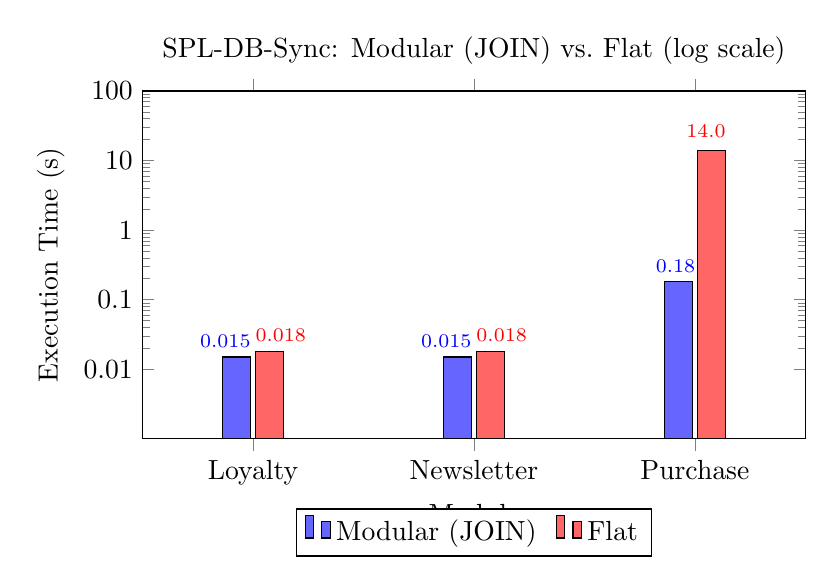
\begin{tikzpicture}
  \begin{axis}[
      ybar,
      width=10cm,
      height=6cm,
      enlarge x limits=0.25,
      symbolic x coords={Loyalty,Newsletter,Purchase},
      xtick=data,
      xlabel={Module},
      ylabel={Execution Time (s)},
      title={SPL-DB-Sync: Modular (JOIN) vs.\ Flat (log scale)},
      ymode=log,
      ymin=1e-3,                        % slightly below smallest bar
      ymax=1e2,                         % space above Purchase bar
      log origin=infty,
      log ticks with fixed point,
      ytick={1e-2,1e-1,1e0,1e1,1e2},
      yticklabels={0.01,0.1,1,10,100},
      legend style={
        at={(0.5,-0.2)},
        anchor=north,
        /tikz/every even column/.append style={column sep=5pt},
        cells={anchor=center}
      },
      legend columns=2
    ]

    % Modular (JOIN) data:
    \addplot[fill=blue!60] coordinates {
      (Loyalty,0.015)
      (Newsletter,0.015)
      (Purchase,0.18)
    };

    % Flat data:
    \addplot[fill=red!60] coordinates {
      (Loyalty,0.018)
      (Newsletter,0.018)
      (Purchase,14.0)
    };

    % Add x‐shifted labels for Loyalty
    \node at (axis cs:Loyalty,0.015) [anchor=south,font=\scriptsize,blue, xshift=-10pt] {0.015};
    \node at (axis cs:Loyalty,0.018) [anchor=south,font=\scriptsize,red,  xshift=+10pt] {0.018};

    % And for Newsletter
    \node at (axis cs:Newsletter,0.015) [anchor=south,font=\scriptsize,blue, xshift=-10pt] {0.015};
    \node at (axis cs:Newsletter,0.018) [anchor=south,font=\scriptsize,red,  xshift=+10pt] {0.018};

    % Purchase labels (no overlap, so no shift needed)
    \node at (axis cs:Purchase,0.18) [anchor=south,font=\scriptsize,blue, xshift=-7pt] {0.18};
    \node at (axis cs:Purchase,14.0) [anchor=south,font=\scriptsize,red, yshift=1pt, xshift=+4pt] {14.0};

    \legend{Modular (JOIN), Flat}

  \end{axis}
\end{tikzpicture}

\section{Threats to validity}
\label{sec:ch4_threats}